
%(BEGIN_QUESTION)
% Copyright 2007, Tony R. Kuphaldt, released under the Creative Commons Attribution License (v 1.0)
% This means you may do almost anything with this work of mine, so long as you give me proper credit

The following chlorine disinfection system (common to wastewater treatment systems) has a subtle problem the loop's stability changes with the weather.  Influent in this case comes from the discharge of an open aeration lagoon, which collects rainwater during stormy weather but of course does not during dry weather.  

When the influent water flow rate is low, the control system will oscillate.  When the influent water flow rate is high, the system will respond sluggishly:

$$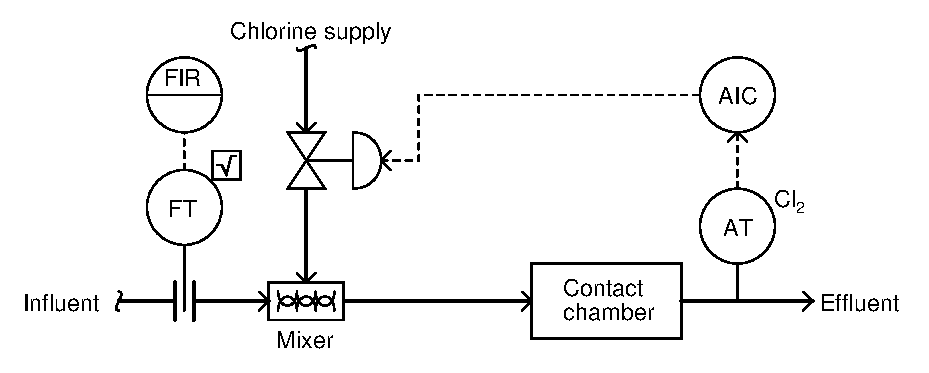
\includegraphics[width=15.5cm]{i01815x02.eps}$$

So far, instrument technicians' approach to solving this problem has been to re-adjust the PID tuning parameters seasonally.  Identify how you think the controller's PID tuning parameters would need to be adjusted between the seasons and wet seasons, being as specific as you can.  Explain {\it why} the process itself seems to control so differently based on influent flow rate.

\vskip 10pt

Explain why the following modification will go a long way toward correcting this problem:

$$\includegraphics[width=15.5cm]{i01815x01.eps}$$

\filbreak

Explain why this next modification works as it does, being an alternative to the former solution:

$$\includegraphics[width=15.5cm]{i01815x03.eps}$$

\underbar{file i01815}
%(END_QUESTION)





%(BEGIN_ANSWER)

The fundamental problem here is that the {\it process gain} varies inversely to flow rate.  During the rainy seasons when the lagoon captures rainwater and the influent flow rate is high, it takes a big change in valve position to make a significant difference in chlorine concentration.  When the weather is dry and the influent flow rate is low, even small moves in valve stem position generate large changes in chlorine concentration.

\vskip 10pt

The multiplication relay (or adaptive gain controller) attempts to keep the overall {\it loop gain} constant despite changes in process gain.

%(END_ANSWER)





%(BEGIN_NOTES)

If you encounter a control system that performs better at one end of its control range than the other, you know you are probably dealing with a variable-gain situation.  The best fix is to make the controller's gain variable in an inverse fashion, so that the overall loop gain remains constant.

%INDEX% Control, PID tuning: process gain (variable)
%INDEX% Control, strategies: adaptive gain
%INDEX% Process: water chlorination

%(END_NOTES)


